\documentclass[11pt]{article}
\usepackage[utf8]{inputenc}
\usepackage[english, ngerman]{babel}
\usepackage{amsmath,amsthm,verbatim,amssymb,amsfonts,amscd}
\usepackage{enumerate}
\usepackage{listings}
\usepackage{courier}
\usepackage[]{graphicx}
\usepackage[]{epstopdf}
\usepackage[margin=1in]{geometry}
\lstset{
  numbers=left,
  language=C,
  basicstyle=\footnotesize\ttfamily,
  breaklines=true,
  morekeywords={function, NIL, new, class, implements, var, true, false}
}
\newcommand{\abs}[1]{\left| #1 \right| }
\setlength{\parindent}{0pt} 

\author{
  Felix Schrader, 3053850 \\ 
  Jens Duffert, 2843110 \\
  Eduard Sauter, 3053470
}
\title{Datenstrukturen und Algorithmen: Haus\"ubung 7}
\begin{document}
\maketitle
\subsection*{Aufgabe 1}
  
  \lstinputlisting{ADTUGraph.js}
  
  \begin{table}[h!]  
  \centering
  \begin{tabular}{|c|c|c|}
  \hline 
  Funktion & Laufzeit & Speicher \\ 
  \hline 
  create & $\mathcal{O}(1)$ & $\mathcal{O}(1)$ \\ 
  \hline 
  nodeValue & $\mathcal{O}(1)$ & $\mathcal{O}(1)$ \\ 
  \hline 
  areAdjacent? & $\mathcal{O}(1)$ & $\mathcal{O}(1)$ \\ 
  \hline 
  edgeWeight & $\mathcal{O}(1)$ & $\mathcal{O}(1)$ \\ 
  \hline 
  iterationStart & $\mathcal{O}(1)$ & $\mathcal{O}(1)$ \\ 
  \hline 
  iterationNext & $\mathcal{O}(1)$ & $\mathcal{O}(1)$ \\ 
  \hline 
  adjacentStart & $\mathcal{O}(\abs{V})$ & $\mathcal{O}(1)$ \\ 
  \hline 
  adjacentNext & $\mathcal{O}(\abs{V})$ & $\mathcal{O}(1)$ \\ 
  \hline 
  insert & $\mathcal{O}(\abs{V})$ & $\mathcal{O}(1)$ \\ 
  \hline 
  remove & $\mathcal{O}(\abs{V}^2)$ & $\mathcal{O}(1)$ \\ 
  \hline 
  changeWeight & $\mathcal{O}(1)$ & $\mathcal{O}(1)$ \\ 
  \hline 
  \end{tabular} 
  \caption{Laufzeiten und Speicherbedarf der Funktionen des ADTÜGraph}
  \label{tab:ADTUGraph}
  \end{table}
  
  In Tabelle \ref{tab:ADTUGraph} wurden die Laufzeiten und Speicher der
  ADTLinkedList aus der Vorlesung verwendet. Laufzeiten über $\mathcal{O}(1)$
  kommen hier durch Iterationen über alle Knoten und die Laufzeit
  $\mathcal{O}(\abs{V})$ von delete hervor.
  
\subsection*{Aufgabe 2}
\begin{enumerate}[a)]
	\item
	In dieser Aufgabe soll der minimale Spannbaum von Punkt A durch das
	Prim-Verfahren bestimmt werden. Dies wurde grafisch dargestellt. Es wurde
	darauf verzichtet, alle Wege bei der Bestimmung farbig zu markieren.\\
	Der Startpunkt ist A. Von A ist es möglich drei Wege zu gehen.
	1.Weg zu D (Wertung 2), 2.Weg zu C (Wertung 9) und 3.Weg zu E (Wertung 9).
	In der Abbildung \ref{fig:a1} links oben ist dies zu sehen.
	\begin{figure}[h!]
		\centering
		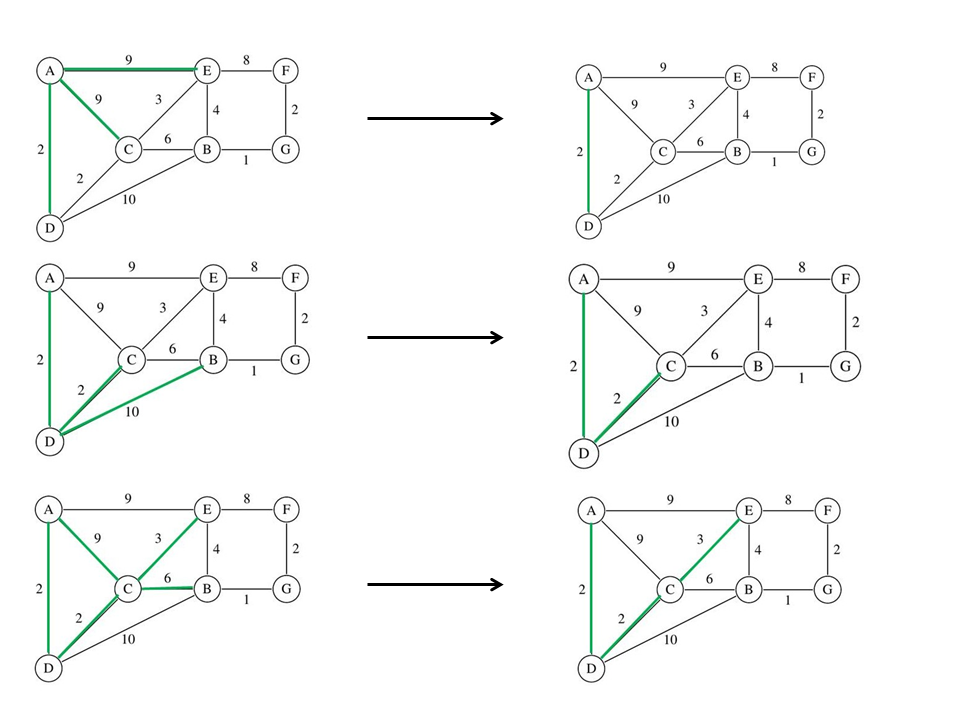
\includegraphics[width=0.8\textwidth]{aufgabe2ateil1.png}
		\caption{Grafik für Verfahren von Prim}
		\label{fig:a1}
	\end{figure}
	Es wird der Weg mit der geringsten Wertung genommen und somit der zu D.
	Von D aus ist es möglich zu C (Wertung 2) und zu B (Wertung 10) zu gelangen.
	Also sind jetzt die Wege zu E, C (je Wertung 9) und zu C (Wertung 2) und B
	(Wertung 10) zur Verfügung. Auch in diesem Fall wird der Weg mit der geringsten
	Wertung genommen. Dies wird mit allen weiteren Wegen gemacht.
	\begin{figure}[h!]
		\centering
		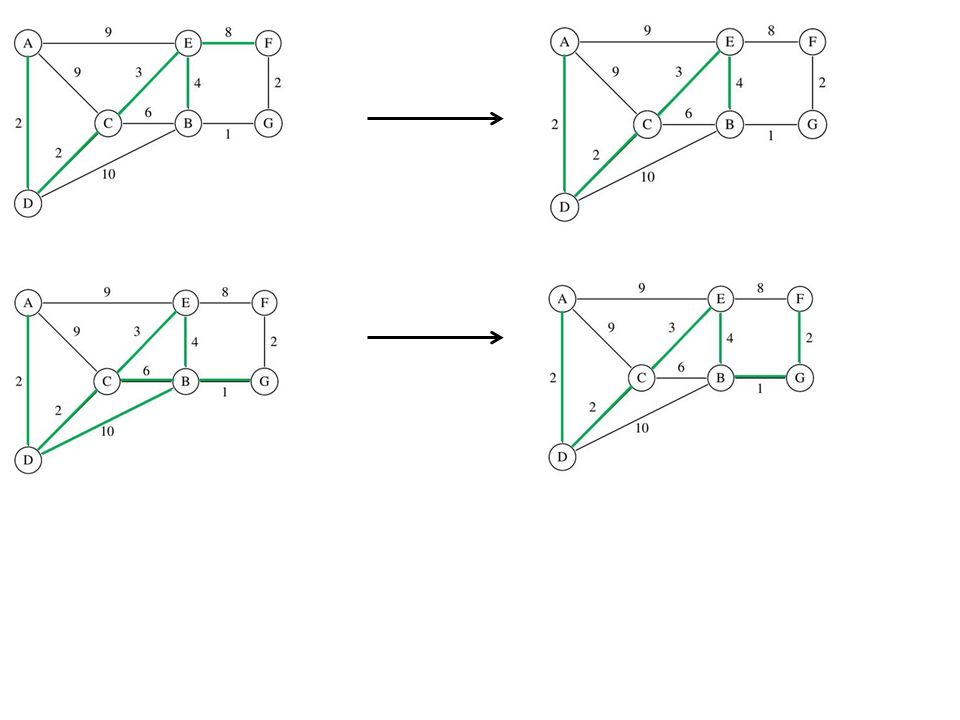
\includegraphics[width=0.8\textwidth]{aufgabe2ateil2.png}
		\caption{Grafik für Verfahren von Prim}
		\label{fig:a2}
	\end{figure}
	Das Ergebnis des minimalen Spannbaum ist in Abbildung \ref{fig:a2} rechts unten
	zu sehen. Dieses lautet:  
	
	
	\begin{align*}
		A \rightarrow D \rightarrow C \rightarrow E \rightarrow B \rightarrow G \rightarrow F
	\end{align*}
	
	
	Dieser hat einen Wert von:
	\begin{align*}
		2 + 2 + 3 + 4 + 1 + 2 = 17
	\end{align*} 
	\newpage
	\item
	Es soll nun mit dem Dijkstra Algorithmus der kürzestes Weg von A zu F bestimmt
	werden. Dabei wurden die ? in den Kästen wo noch keine Informationen vorhanden
	sind weggelassen.
	1.Schritt
	
	\begin{tabular}{|c|c|c|c|c|c|c|c|c|}
		\hline  		  & A & B & C & D & E & F & G & PriorityQueue\\ 
		\hline $dist_{1}$ & 0 &   &  & 2 & 9 &	&  & $D_{2}$\\ 
		\hline $pred_{1}$ & Nil &  &  & A & A &	&  &\\
		\hline 
	\end{tabular} 
	
	2.Schritt
	
	\begin{tabular}{|c|c|c|c|c|c|c|c|c|}
		\hline  		  & A & B & C & D & E & F & G & PriorityQueue\\ 
		\hline $dist_{1}$ & 0 & 12  & 4 & 2 & 9 &  &  & $D_{2}$\\ 
		\hline $pred_{1}$ & Nil & D & D & A & A &  &  &\\
		\hline 
	\end{tabular} 
	
	3.Schritt
	
	\begin{tabular}{|c|c|c|c|c|c|c|c|c|}
		\hline  		  & A & B & C & D & E & F & G & PriorityQueue\\ 
		\hline $dist_{1}$ & 0 & 10  & 4 & 2 & 9 &  &  & $D_{2}$\\ 
		\hline $pred_{1}$ & Nil & C & D & A & A &  &  &\\
		\hline 
	\end{tabular}  
	
	4.Schritt
	
	\begin{tabular}{|c|c|c|c|c|c|c|c|c|}
		\hline  		  & A & B & C & D & E & F & G & PriorityQueue\\ 
		\hline $dist_{1}$ & 0 & 10  & 4 & 2 & 7 & 15 &  & $D_{2}$\\ 
		\hline $pred_{1}$ & Nil & C & D & A & C & E &  &\\
		\hline 
	\end{tabular}
	
	Dies Ergebnis ist nicht effektiv da der kürzestes Weg 14 (Aufgabenteil a) ist und nicht 15 wie mit diesem Algorithmus
	
	
\end{enumerate}   
  
\newpage
  
\section*{Aufgabe 3}
\begin{enumerate}[a)]

  \item Die \emph{graphlib} von cpettit. Hier eine Zusammenfassung des
    Abschnittes ``Graph Concepts'' aus der Dokumentation:
    \begin{description}
      \item[Directed] 
        Dies ist der Standard-Typ. Die Kanten sind gerichtet.

        \begin{figure}[h!]
          \centering
          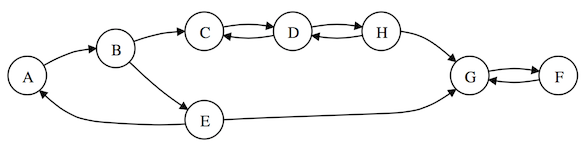
\includegraphics[width=0.5\textwidth]{./tarjan.png}
          \label{fig:}
        \end{figure}

      \item[Undirected]
        Diese sind analog zu denen in der Vorlesung.

        \begin{figure}[h!]
          \centering
          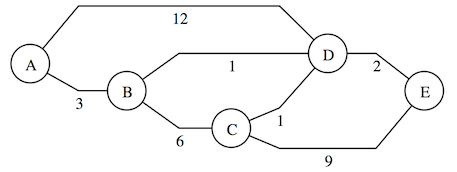
\includegraphics[width=0.5\textwidth]{prim-input.png}
          \label{fig:input}
        \end{figure}

      \item[Multigraph]
        Hier k\"onnen mehrere Kanten zwei gleiche Knoten verbinden. Nicht
        zu verwechseln mit einem ``Hypergraphen'', bei dem eine Kante mehrere
        Knoten verbinden kann.

        \begin{figure}[h!]
          \centering
          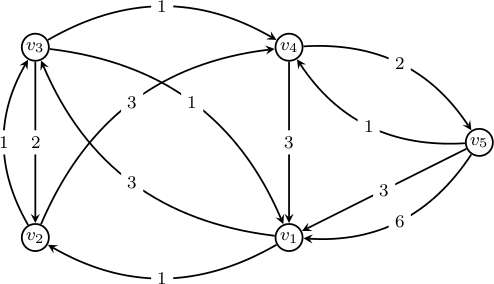
\includegraphics[width=0.5\textwidth]{weighted-multigraph.png}
          \label{fig:multigraph}
        \end{figure}

      \item[Compound]
        Diese sind wie B\"aume mit Wurzeln. Es l\"asst sich eine Kind-Elternteil
        Hirarchie auf den Knoten beschreiben.

        \begin{figure}[h!]
          \centering
          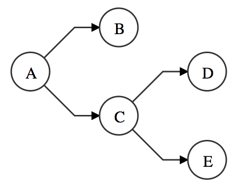
\includegraphics[width=0.3\textwidth]{preorder.png}
          \label{fig:preorder}
        \end{figure}
        
        
        \end{description}
\newpage

      \item \emph{Der Tarjan Algorithmus} \\
        Das Ziel dieses Algorithmus' ist es, die starken Zusammenhangskomponenten
        eines gerichteten Graphen zu bestimmen. Der folgende Code ist aus
        cpettitt's graphlib entnommen:
        \lstinputlisting{tarjan.js}

        Der Algorithmus \"ahnelt der in der Vorlesung besprochenen Tiefensuche,
        Die Buchf\"uhrung des Algorithmus ist jedoch abgewandelt. Es gibt noch
        die zus\"atzlich die Variablen
        \begin{itemize}
          \item \texttt{stack}
          \item \texttt{v.onStack}
          \item \texttt{v.index}
          \item \texttt{v.lowlink}
        \end{itemize}
        Es ist der Index die Reihenfolge, in denen die
        Knoten besucht wurden, dieser entspricht wieder genau dem der Tiefensuche.
        In \texttt{lowlink} ist jetzt jedoch auch die Information enthalten
        welcher Index von einem Knoten aus erreichbar ist. Wenn ein Knoten $a$
        sich auf dem Stack unter einem anderen Knoten $b$ befindet, dann gibt
        es einen Pfad $a \to b$. Dies impliziert auch, dass \texttt{a.index <
        b.index} ist.  Falls umgekehrt \texttt{b.lowlink  == a.lowlink} dann
        gibt es auch einen Pfad $b \to a$.

        Diese \"Uberlegung begr\"undet Zeile 19-20 des Algorithmus: Wenn
        ein Knoten ``grau'' ist, also auf dem Stack, und der \texttt{lowlink}
        des Knoten auf dem Stack kleiner ist, dann haben wir einen Pfad zu-
        und von diesem Knoten gefunden, der \texttt{lowlink} des 
        momentanen Knotens wird also herabgesetzt und der Knoten wird
        als Teil der starken Zusammenhangskomponente, in welcher der Knoten
        auf dem Stack ist, vermerkt. Salopp gesagt ``sucht'' der Algorithmus
        den niedrigsten Index eines anderen Knotens auf dem Stack der von
        diesem aus erreichbar ist. Wenn ein niedrigerer Index als
        \texttt{v.lowlink} gefunden wird, dann ist der Knoten Teil einer
        Zusammenhangskomponente welcher zurzeit in Bearbeitung ist.

        Die Knoten werden also in Reihenfolge ihrer Besuchung auf den Stack
        getan. Wenn am Ende des Funktionsaufrufs kein Knoten mit
        geringerem Index gefunden wurde, dann werden alle Knoten \"uber
        dem jetztigen auf dem Stack als Teil dessen starker
        Zusammenhangskomponente erachtet und vom Stack genommen. Die Knoten
        ``bleiben'' also nur dann auf dem Stack, wenn sie in einer
        Zusammenangskomponente eines anderen Knoten auf dem Stack sind.
        
        Man kann den ersten besuchten Knoten einer starken
        Zusammenhangskomponente auszeichnen, da er den geringsten Index
        besitzt. Nur f\"ur einen solchen Knoten kann \texttt{lowlink  == index}
        gelten. Wenn dies nun am Ende des Aufrufs von \texttt{dfs} gilt, dann
        sind alle Knoten \"uber der Wurzel auf dem Stack in einer Starken
        Zusammenhangskomponente mit dieser. Die Zusammenhangskomponenten haben
        also alle ihren eigenen \texttt{index}, welcher durch den Index des
        ersten besuchten Knotens der Komponente gegeben ist.







\end{enumerate} 


\end{document}
